% =============================================================================
% COPYRIGHT AND DISCLAIMER
% =============================================================================
% This file is provided as a convenience template for competition participants.
% By using it, you accept full responsibility for compliance with all applicable
% copyright, licensing, and usage rules of the Association for Computing
% Machinery (ACM) and of any LaTeX packages you load (including, without
% limitation, the "acmart" document class and related ACM materials).
%
% Consult ACM's official publication, template, and copyright policies before
% using this setup for any purpose other than this competition. Do not assume
% that this template may be reused, redistributed, or submitted elsewhere
% without independently verifying ACM's current rules.
%
% Use of the "acmart" class, the "sigconf" option, or ACM-style formatting in
% this template does NOT mean that this report, this competition, its organizers,
% or any resulting PDF is sponsored, endorsed, affiliated with, or published by
% ACM. ACM trademarks and branding remain the property of ACM.
%
% Template packages live in preamble.tex.
% Citations live in main.bib. Edit this file with your paper content.
% =============================================================================

\documentclass[sigconf]{acmart}
% =============================================================================
% Template setup — participants normally do not edit this file.
% Author content belongs in main.tex; citations belong in main.bib.
% \documentclass lives in main.tex so Overleaf does not treat this file as root.
% =============================================================================

% --- Competition / non-ACM-submission friendly rights metadata -------------
\setcopyright{none}
\settopmatter{printacmref=false}
\acmConference[Kaggle Competition]{Filament Segmentation Challenge}{2026}{\href{https://www.kaggle.com/competitions/filament-segmentation-2026}{kaggle.com/competitions/filament-segmentation-2026}}
\acmBooktitle{Competition Report}
\acmDOI{}
\acmISBN{}

% --- Author guidance text --------------------------------------------------
% \guide{...} is gray italic while \guideStyletrue; omitted from the PDF if false.
% Flip the switch in main.tex after % =============================================================================
% Template setup — participants normally do not edit this file.
% Author content belongs in main.tex; citations belong in main.bib.
% \documentclass lives in main.tex so Overleaf does not treat this file as root.
% =============================================================================

% --- Competition / non-ACM-submission friendly rights metadata -------------
\setcopyright{none}
\settopmatter{printacmref=false}
\acmConference[Kaggle Competition]{Filament Segmentation Challenge}{2026}{\href{https://www.kaggle.com/competitions/filament-segmentation-2026}{kaggle.com/competitions/filament-segmentation-2026}}
\acmBooktitle{Competition Report}
\acmDOI{}
\acmISBN{}

% --- Author guidance text --------------------------------------------------
% \guide{...} is gray italic while \guideStyletrue; omitted from the PDF if false.
% Flip the switch in main.tex after % =============================================================================
% Template setup — participants normally do not edit this file.
% Author content belongs in main.tex; citations belong in main.bib.
% \documentclass lives in main.tex so Overleaf does not treat this file as root.
% =============================================================================

% --- Competition / non-ACM-submission friendly rights metadata -------------
\setcopyright{none}
\settopmatter{printacmref=false}
\acmConference[Kaggle Competition]{Filament Segmentation Challenge}{2026}{\href{https://www.kaggle.com/competitions/filament-segmentation-2026}{kaggle.com/competitions/filament-segmentation-2026}}
\acmBooktitle{Competition Report}
\acmDOI{}
\acmISBN{}

% --- Author guidance text --------------------------------------------------
% \guide{...} is gray italic while \guideStyletrue; omitted from the PDF if false.
% Flip the switch in main.tex after \input{preamble}.
%
% Do not use \guide{...} for \email{...}.
\usepackage{xcolor}
\newif\ifguideStyle
\guideStyletrue
\newcommand{\guide}[1]{%
  \ifguideStyle
    {\color{gray!65}\itshape #1}%
  \fi
}

% --- Math ------------------------------------------------------------------
% Do NOT load amssymb (or amsfonts): acmart already loads newtxmath, which
% defines the same symbols (e.g. \Bbbk) and causes a conflict on Overleaf.
% amsmath is already provided by acmart; mathtools extends it.
\usepackage{mathtools}

% --- Figures ---------------------------------------------------------------
% graphicx is already loaded by acmart
\usepackage{subcaption}

% --- Tables ----------------------------------------------------------------
% booktabs is already loaded by acmart
\usepackage{tabularx}
\usepackage{multirow}

% --- Bibliography style is set in main.tex (ACM-Reference-Format) ----------
.
%
% Do not use \guide{...} for \email{...}.
\usepackage{xcolor}
\newif\ifguideStyle
\guideStyletrue
\newcommand{\guide}[1]{%
  \ifguideStyle
    {\color{gray!65}\itshape #1}%
  \fi
}

% --- Math ------------------------------------------------------------------
% Do NOT load amssymb (or amsfonts): acmart already loads newtxmath, which
% defines the same symbols (e.g. \Bbbk) and causes a conflict on Overleaf.
% amsmath is already provided by acmart; mathtools extends it.
\usepackage{mathtools}

% --- Figures ---------------------------------------------------------------
% graphicx is already loaded by acmart
\usepackage{subcaption}

% --- Tables ----------------------------------------------------------------
% booktabs is already loaded by acmart
\usepackage{tabularx}
\usepackage{multirow}

% --- Bibliography style is set in main.tex (ACM-Reference-Format) ----------
.
%
% Do not use \guide{...} for \email{...}.
\usepackage{xcolor}
\newif\ifguideStyle
\guideStyletrue
\newcommand{\guide}[1]{%
  \ifguideStyle
    {\color{gray!65}\itshape #1}%
  \fi
}

% --- Math ------------------------------------------------------------------
% Do NOT load amssymb (or amsfonts): acmart already loads newtxmath, which
% defines the same symbols (e.g. \Bbbk) and causes a conflict on Overleaf.
% amsmath is already provided by acmart; mathtools extends it.
\usepackage{mathtools}

% --- Figures ---------------------------------------------------------------
% graphicx is already loaded by acmart
\usepackage{subcaption}

% --- Tables ----------------------------------------------------------------
% booktabs is already loaded by acmart
\usepackage{tabularx}
\usepackage{multirow}

% --- Bibliography style is set in main.tex (ACM-Reference-Format) ----------


% Guide styling: \guideStyletrue = show gray italic hints; \guideStylefalse = omit them
\guideStylefalse

\begin{document}

\title{ThreadNet}
\subtitle{A Solution to the Solar Filament Segmentation Challenge 2026} % DO NOT CHANGE


\author{Jose P. Marchezi}
\affiliation{%
  \institution{National Institute for Space Research (INPE)}
  \city{São José dos Campos}
  \country{Brazil}
}
\email{jpmarchezi@gmail.com}

\begin{abstract}
    This report describes our solution to the Solar Filament Segmentation Challenge~2026, a Kaggle competition on automatic segmentation of solar filaments in GONG H-$\alpha$ observations. Our pipeline, ThreadNet, detects filaments with a YOLO11 object detector, refines each detected region with a compact edge-attention U-Net, and stitches the resulting crop-level masks back into a full-resolution instance map with a greedy, confidence-ordered mask-level non-maximum suppression. We explore five independent extensions to this baseline -- $k$-fold cross-validation with copy-paste augmentation, oriented bounding boxes, model ensembling with a classical (non-learned) detector, photometric normalization, and flip-based test-time augmentation (TTA) -- and report which of them survive validation. Only topology-safe flip-4 TTA improves on the baseline, raising the pooled Panoptic Quality (PQ) from 0.4381 to 0.4405 on our held-out validation split, comfortably above the organizers' stated threshold of practical value (PQ~$>$~0.35).
\end{abstract}

\maketitle

% ==================================== %
%              INTRODUCTION            %
% ==================================== %
\section{Introduction}
    This report goes over the details of our submitted solution to the Solar Filament Segmentation Challenge~2026 \cite{filament-segmentation-2026}. The challenge, launched on July~10,~2026, is organized by the Earth-Space AI Research (ESAIR) Lab\footnote{\href{https://www.esairlab.com/home}{www.esairlab.com/}}. This challenge utilizes the MAGFiLO dataset for evaluation of the segmentation algorithms \cite{ahmadzadeh2024dataset}.

    Rather than a single novel architecture, our contribution is a systematic search over the space of reasonable extensions to a strong detect-then-segment baseline, each validated in isolation against the same held-out split before being adopted or discarded. Section~\ref{sec:methodology} describes the adopted pipeline, ThreadNet, and the extensions we tested; Section~\ref{sec:evaluation} reports which of them actually improved Panoptic Quality (PQ), the competition's ranking metric, and discusses the failure modes that remain.


% ==================================== %
%              METHODOLOGY             %
% ==================================== %
\section{Methodology}\label{sec:methodology}

\subsection{Pipeline overview}
    ThreadNet follows a detect-crop-refine design (Figure~\ref{fig:pipeline}). A YOLO11s object detector \cite{jocher2023yolo}, trained on the full-disk image downsampled to $1024\times1024$, proposes an axis-aligned bounding box per candidate filament. Each box is padded (by a factor of $1.35\times$ its size, or a minimum of 48\,px) and letterbox-resized to a $256\times256$ crop that preserves the filament's native aspect ratio -- an important detail, since filaments are long and thin, and a naive square crop wastes most of its resolution on empty margin once resized. A compact U-Net (8.8M parameters, base width 32) with an edge-guided self-attention bottleneck \cite{ronneberger2015unet, solomon2025edgeattnet} then predicts a binary mask for the crop; the edge-attention mechanism biases the bottleneck's Query/Key projections with a learned edge map of the input crop, which helps recover the thin, low-contrast barbs that branch off a filament's main spine.

    Each crop-level mask is un-letterboxed back to its native resolution and pasted into the full $2048\times2048$ label map. Because ordinary box-level non-maximum suppression is a poor proxy for ``same object'' on long, thin, diagonal filaments, instances are merged with a \emph{mask-level} greedy NMS instead: candidates are processed in decreasing detection confidence, and a candidate is rejected outright if it is already mostly covered by a higher-confidence instance, rather than accepted as a fragment.

    \begin{figure}[t]
      \centering
      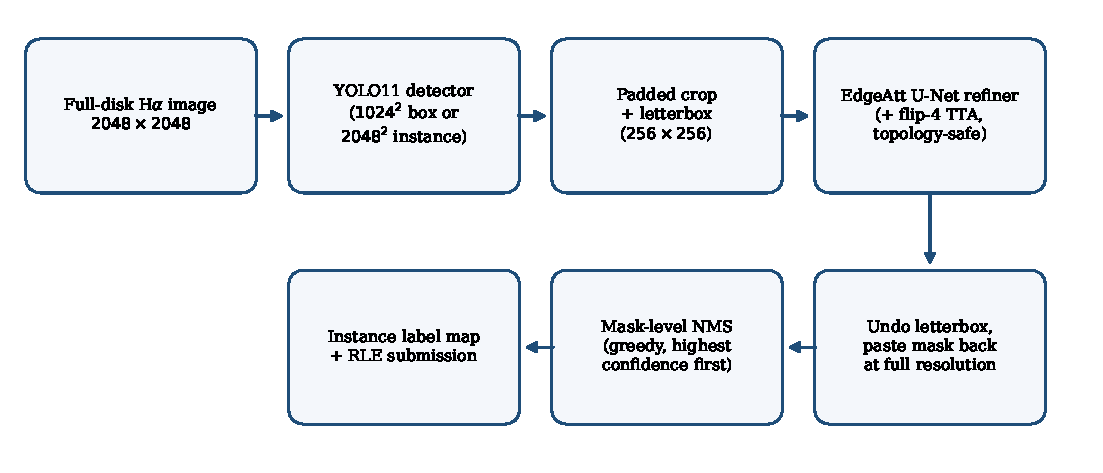
\includegraphics[width=\linewidth]{figures/pipeline.pdf}
      \caption{ThreadNet's inference pipeline: detect, crop, refine (with optional flip-4 TTA), un-letterbox, and stitch via mask-level NMS.}
      \Description{Six-box flow diagram showing a full-disk H-alpha image processed by a YOLO11s detector, then a padded and letterboxed crop, then a U-Net refiner with test-time augmentation, then undone letterboxing, mask-level non-maximum suppression, and a final instance label map.}
      \label{fig:pipeline}
    \end{figure}

\subsection{Data and sampling strategy}
    We use the MAGFiLO dataset \cite{ahmadzadeh2024dataset}, which contains 707 image records over a smaller number of unique physical images -- up to three independent annotators can label the same photograph, each producing a separate image record under a distinct identifier that shares one underlying \texttt{file\_name}. All train/validation splits are therefore performed at the level of the physical image, not the image record: splitting on the record identifier alone would leak the same photograph's pixels into both splits whenever it carried multiple annotator records. Our reported results use a single 90/10 split at this granularity; during development we additionally used 5-fold cross-validation (same leak-safe grouping) to obtain a low-variance PQ estimate before committing to any given change.

    The U-Net is trained on independently cropped filaments (one crop per annotation) with random horizontal/vertical flips, a random $90^\circ$ rotation, and gamma correction ($\gamma \sim U(0.5, 1.5)$, applied with probability 0.9) for invariance to nonlinear brightness variation -- motivated by a real, measured limb-darkening gradient in this dataset (mean on-disk intensity falls from about 140 near disk center to about 76 near the limb) and matching the augmentation recipe of \citet{hu2026modernconvnet}. The YOLO detector is trained with flips and mild rotation/scale/translation jitter; mosaic augmentation and all color jitter are disabled, since these are single-channel grayscale observations.

\subsection{Extensions explored}
    Beyond this baseline, we implemented and validated five independent extensions, each toggleable in isolation:
    \begin{itemize}
        \item \textbf{$k$-fold CV + copy-paste augmentation}: synthetic training images built by pasting real filament patches (their own polygon mask, feathered and brightness-matched) onto other on-disk backgrounds, away from existing ground truth.
        \item \textbf{Oriented bounding boxes (OBB)}: a YOLO11s-obb detector predicting the filament's orientation directly, with a single-pass rotate-crop-segment-unrotate inference path.
        \item \textbf{Model ensembling}: merging the axis-aligned and OBB pipelines, and a classical, non-learned Shih-and-Kowalski-style detector (local-median thresholding and multi-directional morphological closing), via the same mask-level NMS used for stitching, applied across sources instead of within one.
        \item \textbf{Photometric normalization}: dividing each on-disk pixel by its smoothed radial-average intensity to flatten limb darkening, followed by CLAHE, applied to both detector and refiner inputs; and InstanceNorm in place of BatchNorm in the U-Net, following \citet{hu2026modernconvnet}.
        \item \textbf{Flip-4 test-time augmentation (TTA)}: at inference, the U-Net's probability map is averaged over the identity, horizontal-flip, vertical-flip, and both-flip views of a crop. The average is trusted only if it does not change the single-view mask's topology: its area must stay within $[0.6, 1.7]\times$ the single-view area, its connected-component count must not grow by more than one, and (once the single-view mask is large enough for the comparison to be meaningful) its Dice overlap against the single-view mask must be at least 0.62. Otherwise, inference falls back to the plain single-view mask. This guard is what makes the technique safe to compose with everything else in the pipeline: it can only remove noise from a prediction, never introduce a qualitatively different one.
    \end{itemize}
    Section~\ref{sec:evaluation} reports that only the last of these, flip-4 TTA, improved PQ over the baseline; the others are retained in our public repository as validated negative results.


% ==================================== %
%              EVALUATION              %
% ==================================== %
\section{Evaluation}\label{sec:evaluation}

\subsection{Evaluation strategy}
    We reproduce the organizers' own Panoptic Quality (PQ) computation locally: predicted and ground-truth instances are matched globally (not per image) by IoU~$>$~0.5, and $\mathrm{PQ} = \sum \mathrm{IoU}(\mathrm{TP}) / (|\mathrm{TP}| + 0.5|\mathrm{FP}| + 0.5|\mathrm{FN}|)$, pooling true/false positives and negatives across the entire validation set rather than averaging a per-image score -- a stricter, more punishing aggregation than a naive per-image mean. Every configuration below was re-tuned over its own detection-confidence threshold before being trusted, since we found repeatedly that a threshold tuned for one model configuration transfers poorly to another.

\subsection{Results across explored configurations}
    Table~\ref{tab:results} summarizes PQ on our held-out validation split for the baseline and every extension from Section~\ref{sec:methodology}. Four of the five extensions plateaued at or below the baseline; only flip-4 TTA improved it, and by a modest but reproducible margin across two independently swept mask-merge thresholds.

    \begin{table}[t]
      \centering
      \caption{PQ across explored configurations (held-out validation split).}
      \label{tab:results}
      \begin{tabular}{lc}
        \toprule
        Configuration & PQ \\
        \midrule
        Axis-aligned baseline (YOLO11s + U-Net) & 0.4381 \\
        \quad + 5-fold CV + copy-paste augmentation & 0.4368 \\
        \quad + Oriented bounding boxes (OBB) & 0.4207 \\
        \quad + Ensemble (axis-aligned + OBB) & 0.4321 \\
        \quad + Photometric normalization (limb + CLAHE) & 0.4248 \\
        \quad + InstanceNorm & 0.4345 \\
        \quad + Flip-4 topology-safe TTA (\textbf{adopted}) & \textbf{0.4405} \\
        \bottomrule
      \end{tabular}
    \end{table}

    Our final configuration (axis-aligned baseline with flip-4 TTA) resolves 399 true-positive matches against 674 ground-truth filaments, at a mean IoU of 0.690 among matches and a mean Dice of 0.739 among any nonzero overlap (Figure~\ref{fig:distributions}). Instance-level fragmentation is low: only 2.1\% of ground-truth filaments are split across multiple predictions, and only 3.8\% of predictions merge more than one ground-truth filament, indicating that the mask-level NMS is doing its job of keeping instances cleanly separated.

    \begin{figure}[t]
      \centering
      \begin{minipage}{0.49\linewidth}
        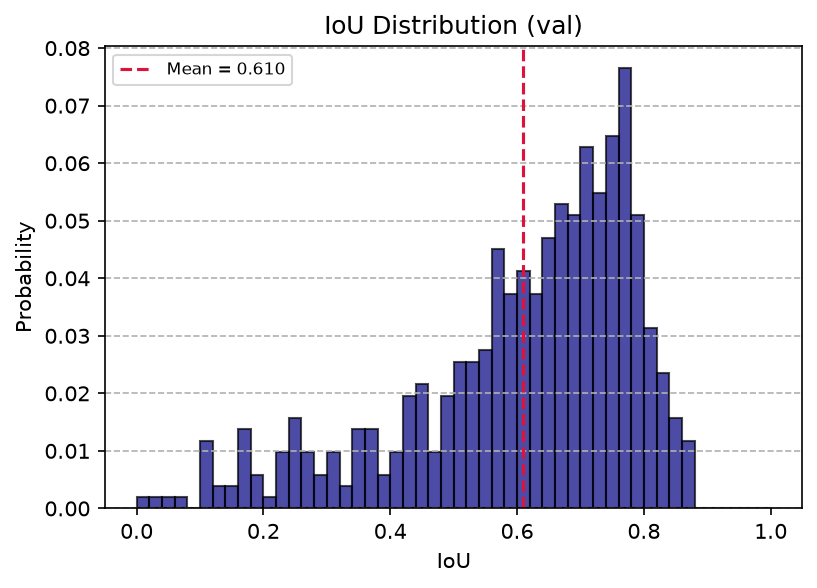
\includegraphics[width=\linewidth]{figures/iou_distribution.png}
      \end{minipage}\hfill
      \begin{minipage}{0.49\linewidth}
        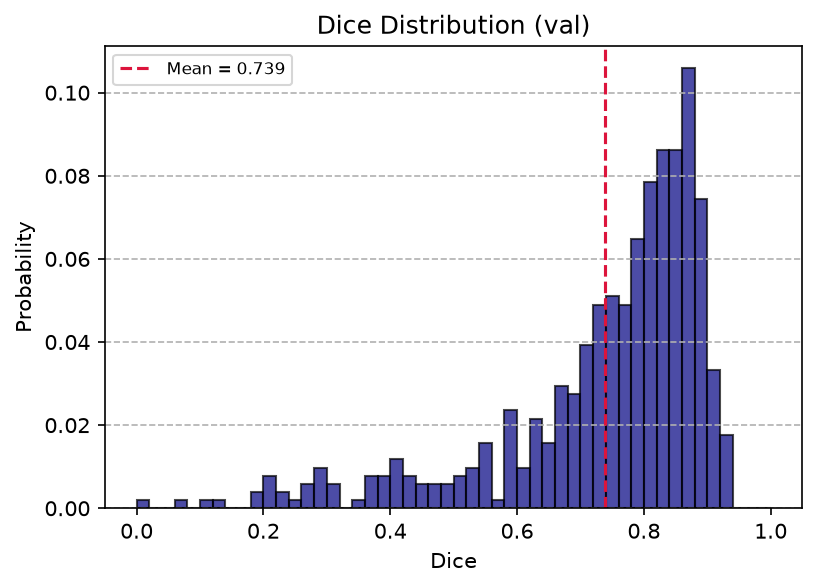
\includegraphics[width=\linewidth]{figures/dice_distribution.png}
      \end{minipage}
      \caption{IoU and Dice distributions over all matched ground-truth/prediction pairs, final configuration.}
      \Description{Two histograms, side by side. The left shows the distribution of IoU scores between matched ground-truth and predicted filament instances, with a mean near 0.69. The right shows the corresponding Dice score distribution, with a mean near 0.74.}
      \label{fig:distributions}
    \end{figure}

    Figure~\ref{fig:examples} shows two representative validation images with predicted instances overlaid against ground truth: agreement is close on well-separated, high-contrast filaments, and the visible disagreements -- a missed short/faint filament, a slightly offset boundary -- are consistent with the quantitative gap described below.

    \begin{figure}[t]
      \centering
      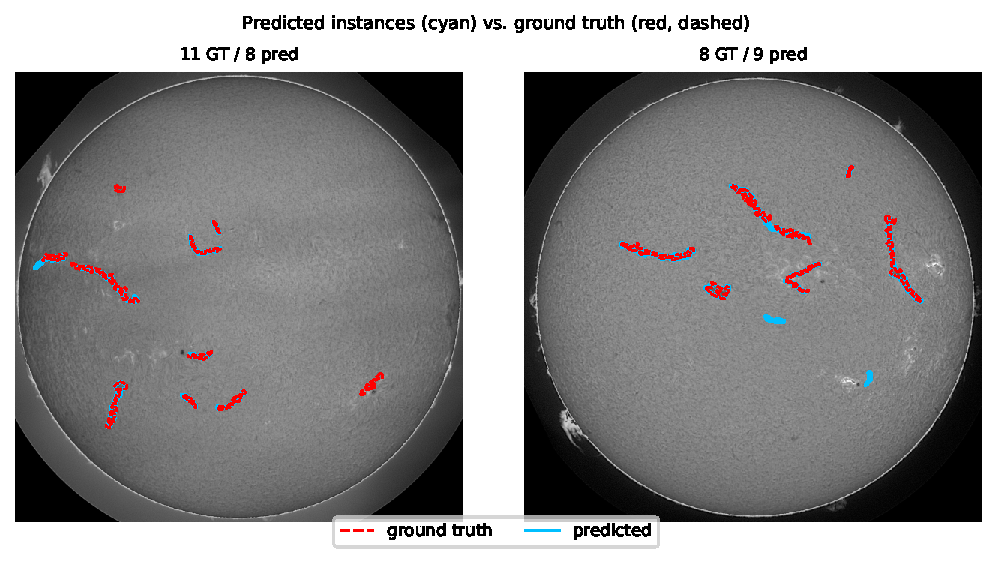
\includegraphics[width=\linewidth]{figures/examples.pdf}
      \caption{Predicted instances (cyan) against ground truth (red, dashed) on two validation images.}
      \Description{Two solar disk images with predicted filament outlines in cyan and ground-truth filament outlines in dashed red, overlaid on the H-alpha image. Most filaments show close agreement between the two outlines, with a few ground-truth filaments left unmatched.}
      \label{fig:examples}
    \end{figure}

\subsection{Strengths, weaknesses, and possible improvements}
    ThreadNet's PQ of 0.4405 is well above the value the organizers themselves flagged as practically meaningful (PQ~$>$~0.35), and the pipeline is modular: mask-level NMS is reused, unmodified, both to merge crop-level predictions into one image and to merge predictions from independent detectors in the ensemble variant, and every extension in Section~\ref{sec:methodology} composes with the others through the same handful of function signatures.

    The main limitation is recall, not mask quality: 26.4\% of ground-truth filaments have no matching prediction at all, while the 15.6\% of predictions with no ground-truth match are comparatively less costly under PQ's aggregation. This is consistent with every extension we tried landing close to the baseline: $k$-fold cross-validation, copy-paste augmentation, an oriented detector, ensembling, and photometric normalization each address mask quality, instance separation, or optimization stability, but none of them directly attacks detector recall on the faintest, shortest filaments -- exactly the failure mode visible in Figure~\ref{fig:examples}. We expect the more promising directions for a future iteration to be ones that target recall directly: additional real (not synthetic) annotated data, an explicit low-confidence recovery pass conditioned on the U-Net's own mask confidence rather than the detector's box confidence alone, or auxiliary supervision on the filament's skeleton/spine to help the detector propose boxes around thin, low-contrast structures it currently misses entirely.



% ==================================== %
%            ACKNOWLEDGMENT            %
% ==================================== %
\section{Acknowledgment}\label{sec:acknowledgment}
    % Do not change
    The organization of the Filament Segmentation Challenge 2026 is partially supported by the U.S. National Science Foundation (NSF) under Grant No. 2209912 and 2433781, directorate for Computer and Information Science and Engineering (CSE), and Office of Advanced Cyberinfrastructure (OAC), and Grant No. 2511630, AST Division Of Astronomical Sciences and MPS Directorate for Mathematical and Physical Sciences.

    The Filament Segmentation Challenge 2026 is sponsored by the U.S. National Science Foundation (NSF) National Solar Observatory (NSO).

    This work utilizes GONG data obtained by the NSO Integrated Synoptic Program, managed by the National Solar Observatory, which is operated by the Association of Universities for Research in Astronomy (AURA), Inc. under a cooperative agreement with the National Science Foundation and with contribution from the National Oceanic and Atmospheric Administration. The GONG network of instruments is hosted by the Big Bear Solar Observatory, High Altitude Observatory, Learmonth Solar Observatory, Udaipur Solar Observatory, Instituto de Astrofísica de Canarias, and Cerro Tololo Interamerican Observatory.

\bibliographystyle{ACM-Reference-Format}
\bibliography{main}

\end{document}
